\cleardoublepage
\lgf{\chapter{Découvrons le LoPy}}
\lge{\chapter{Discover the LoPy}}

\lgf{\textit{Les programmes relatifs à cette section se trouvent dans le répertoire \texttt{plido-tp3} pour le serveur et \texttt{pycom} pour le LoPy.}}
\lge{\textit{The programs related to this section are located in the \texttt{plido-tp3} directory for the server and \texttt{pycom} for the LoPy.}}


\section{Introduction}

\lgf{Grâce aux émulateurs de capteurs décrits au chapitre précédent, vous avez pu appliquer les concepts essentiels de l'IoT sur votre ordinateur.}
\lge{Using the sensor emulators described in the previous chapter, you have been able to apply the essential IoT concepts to your computer.}

\lgf{Cependant, si vous le pouvez, nous vous invitons à le faire sur de vrais objets connectés en utilisant des \Index{LoPy4} (plateforme de prototypage IoT) de la société \Index{Pycom} et des capteurs de température, humidité et pression \Index{BME280} (cf. figure~\vref{fig-lopy-bme280}).}
\lge{However, if you can, we invite you to do it on real connected objects using \Index{LoPy4} (IoT prototyping platform) from the company \Index{Pycom} and temperature, humidity and pressure sensors \Index{BME280} (see figure~\vref{fig-lopy-bme280}).}


\begin{figure}[tbp]
\centerline{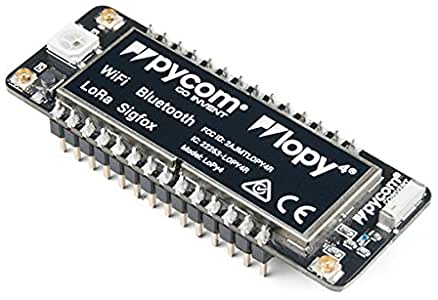
\includegraphics[width=.5\columnwidth]{Pictures/LoPy.jpg}  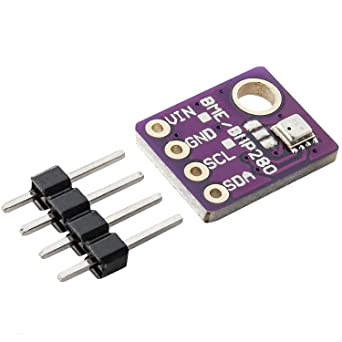
\includegraphics[width=.3\columnwidth]{Pictures/BME280.jpeg}}
\lgf{\caption{LoPY4 et capteur BME280}}
\lge{\caption{LoPY4 and BME280 sensor}}
\label{fig-lopy-bme280}
\end{figure}

\lgf{Un LoPY4 se programme en Python (ou plutôt \Index{micro-python} qui est la version du langage pour systèmes embarqués) pour traiter les données. Dans un premier temps, nous allons utiliser le Wi-Fi pour communiquer avec votre ordinateur mais, par la suite, nous mettrons en place une communication via \Index{LoRaWAN} ou \Index{Sigfox} qui peut vous demander plus de configuration mais vous permettra de mieux comprendre ces protocoles.}
\lge{A LoPY4 is programmed in Python (or rather \Index{micro-python} which is the version of the language for embedded systems) to process data. At first, we will use Wi-Fi to communicate with your computer but, later, we will set up a communication via \Index{LoRaWAN} or \Index{Sigfox} which may require more configuration but will allow you to better understand these protocols.}


     \vspace{1em}


\lgf{Même si vous n’avez pas de LoPy4, vous pouvez parcourir cette section pour voir les contraintes supplémentaires liées aux objets connectés.}
\lge{Even if you don't have LoPy4, you can browse this section to see additional constraints related to connected objects.}


\lgf{\section{Installation d'Atom}}
\lge{\section{Installing Atom}}


\lgf{\Index{Atom} est un éditeur de texte performant, spécifiquement conçu pour le codage en différents langages. 
Atom va nous aider à programmer en Python et va également gérer la communication avec notre LoPy via le port \Index{USB} (grâce au plugin \Index{pymakr}). 
Atom fonctionne à peu près de la même manière sur \Index{Mac OS}, \Index{Windows} et \Index{Linux}, mais en s’adaptant aux particularités du système d’exploitation (place dans les menus, nom des liens séries...). 
Donc, il se peut que vous ayez quelques différences entre ce que vous avez dans cet ouvrage et l’écran de votre ordinateur. 
Les menus et sites Web indiqués peuvent également changer au cours du temps même si nous nous efforçons de faire des mises à jour régulières du cours.}
\lge{\Index{Atom} is a powerful text editor, specifically designed for coding in different languages. 
Atom will help us to program in Python and will also manage the communication with our LoPy via the \Index{USB} (thanks to the plugin \Index{pymakr}). 
Atom works in much the same way on \Index{Mac OS}, \Index{Windows} and \Index{Linux}, but it adapts to the particularities of the operating system (place in the menus, name of the serial links...). 
So, you may have some differences between what you have in this book and the screen of your computer. 
The menus and websites shown may also change over time, although we try to update the course regularly.}


     \vspace{1em}

\lgf{Pour commencer à programmer avec votre LoPy, vous devez installer sur votre ordinateur le logiciel Atom (voir sur \url{http://atom.io}). 
Vous pouvez télécharger le package correspondant à votre système d'exploitation (cf. figure suivante).}
\lge{To start programming with your LoPy, you must install on your computer the Atom software (see \url{http://atom.io}). 
You can download the package corresponding to your operating system (see next figure).}


\begin{figure}[tbp]
\centerline{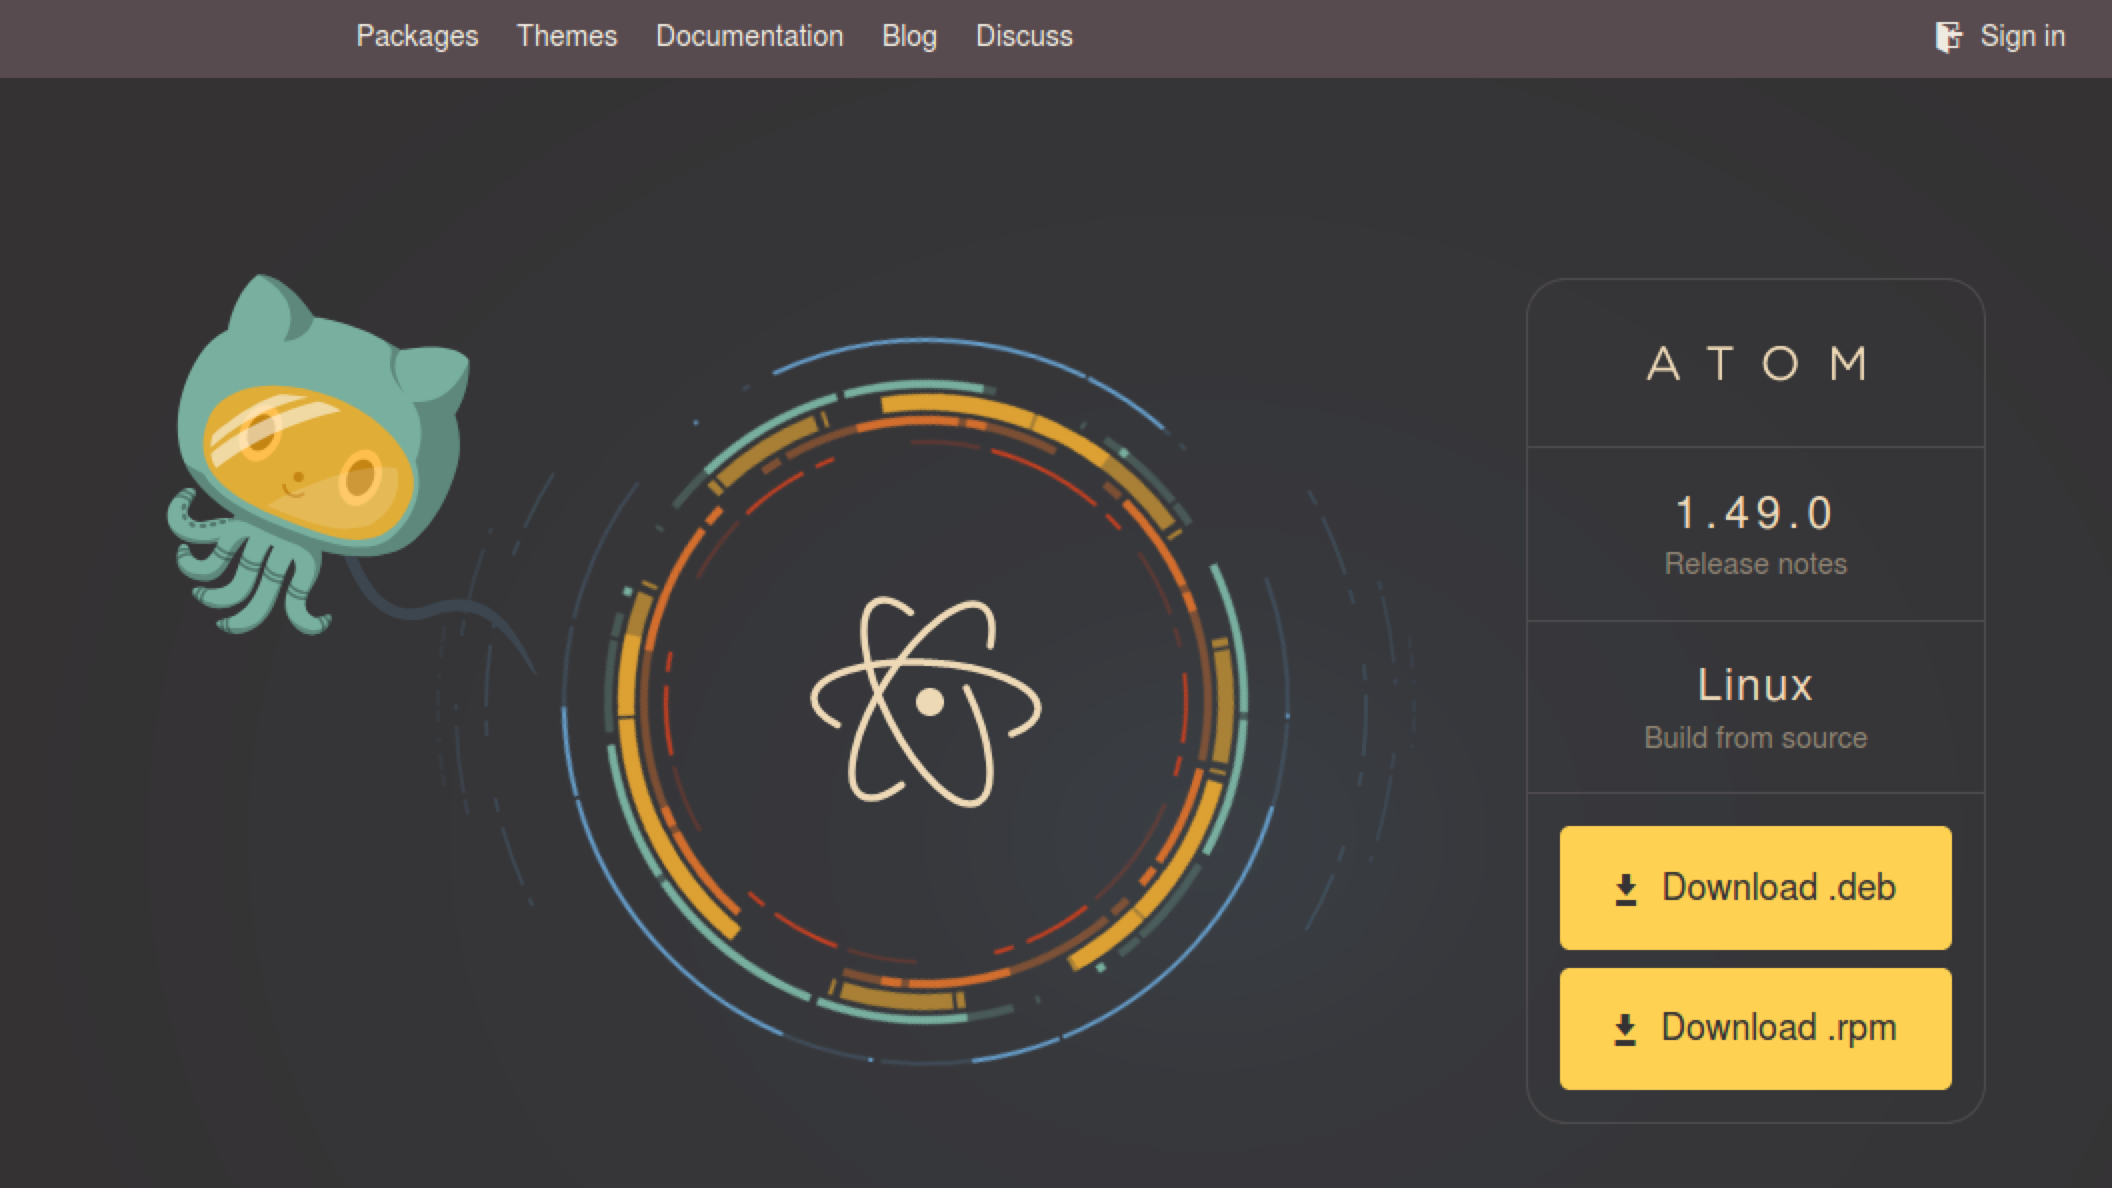
\includegraphics[width=1\columnwidth]{Pictures/atom_dl.png}}
\lgf{\caption{Page d'accueil d'Atom}}
\lge{\caption{Atom homepage}}
\label{fig-page-atom}
\end{figure}


\begin{itemize}
\item 
    \lgf{Pour Mac et Windows, cliquez sur l’icône "télécharger" pour l’installer\footnote{il y a des risques d'incompatibilité des dernières versions d'Atom avec le package de gestion du LoPy (pymakr). Nous vous recommandons d'utiliser une version plus ancienne, comme la 1.43 disponible dans les archives d'Atom Release \url{https://github.com/atom/atom/releases/tag/v1.43.0}(\texttt{AtomSetup-x64.exe} pour Windows ou \texttt{atom-mac.zip} pour Mac OS).}.}
    \lge{For Mac and Windows, click on the "download" icon to install it. There is a risk of incompatibility between the latest versions of Atom and the LoPy management package (pymakr). We recommend you to use an older version, like the 1.43 available in the Atom Release archives (\url{https://github.com/atom/atom/releases/tag/v1.43.0}(\texttt{AtomSetup-x64.exe} for Windows or \texttt{atom-mac.zip} for Mac OS).}    
\item 
    \lgf{Pour Linux, téléchargez le\texttt{.deb} et tapez \texttt{sudo dpkg -i atom-amd64.deb}\footnote{Il est possible qu'un message vous dise que git n'est pas installé. Dans ce cas, tapez \texttt{sudo apt-get install git} et suivez les instructions).}.
    Lancez Atom en cliquant sur l’icône ou, sous Linux, en tapant atom dans un terminal.}
    \lge{For Linux, download letexttt{.deb} and type \texttt{sudo dpkg -i atom-amd64.deb}\footnote{It is possible that a message tells you that git is not installed. In this case, type \texttt{sudo apt-get install git} and follow the instructions}.
    Launch Atom by clicking on the icon or, under Linux, by typing atom in a terminal.}
\end{itemize}

     \vspace{1em}

\lgf{Lancez Atom en cliquant sur l’icône ou, sous Linux, en tapant atom dans un terminal. L’écran d’accueil apparaît.}
\lge{Launch Atom by clicking on the icon or, under Linux, by typing atom in a terminal. The welcome screen appears.}


\lgf{\subsection{Communiquez avec votre Pycom}}
\lge{\subsection{Communicate with your Pycom}}


\lgf{Pour communiquer avec le Pycom à travers Atom, vous devez installer le package \texttt{\Index{pymakr}}.}
\lge{To communicate with the Pycom through Atom, you must install the \texttt{\Index{pymakr}} package.}

\lgf{Cliquez sur \textit{Install a Package} puis \textit{Open Installer}. Une autre fenêtre s’ouvre (cf. figure~\vref{fig-page-pakage}. Tapez \texttt{pymakr} dans le menu. Un package apparaît portant ce nom. Cliquez sur \textit{Install}. L’installation peut prendre plusieurs minutes. Vous avez le temps de prendre un café.}
\lge{Click on \textit{Install a Package} then \textit{Open Installer}. Another window will open (see figure~\vref{fig-page-pakage}. Type \texttt{pymakr} in the menu. A package with this name appears. Click on \textit{Install}. The installation may take several minutes. You have time to have a coffee.}


\begin{figure}[tbp]
\centerline{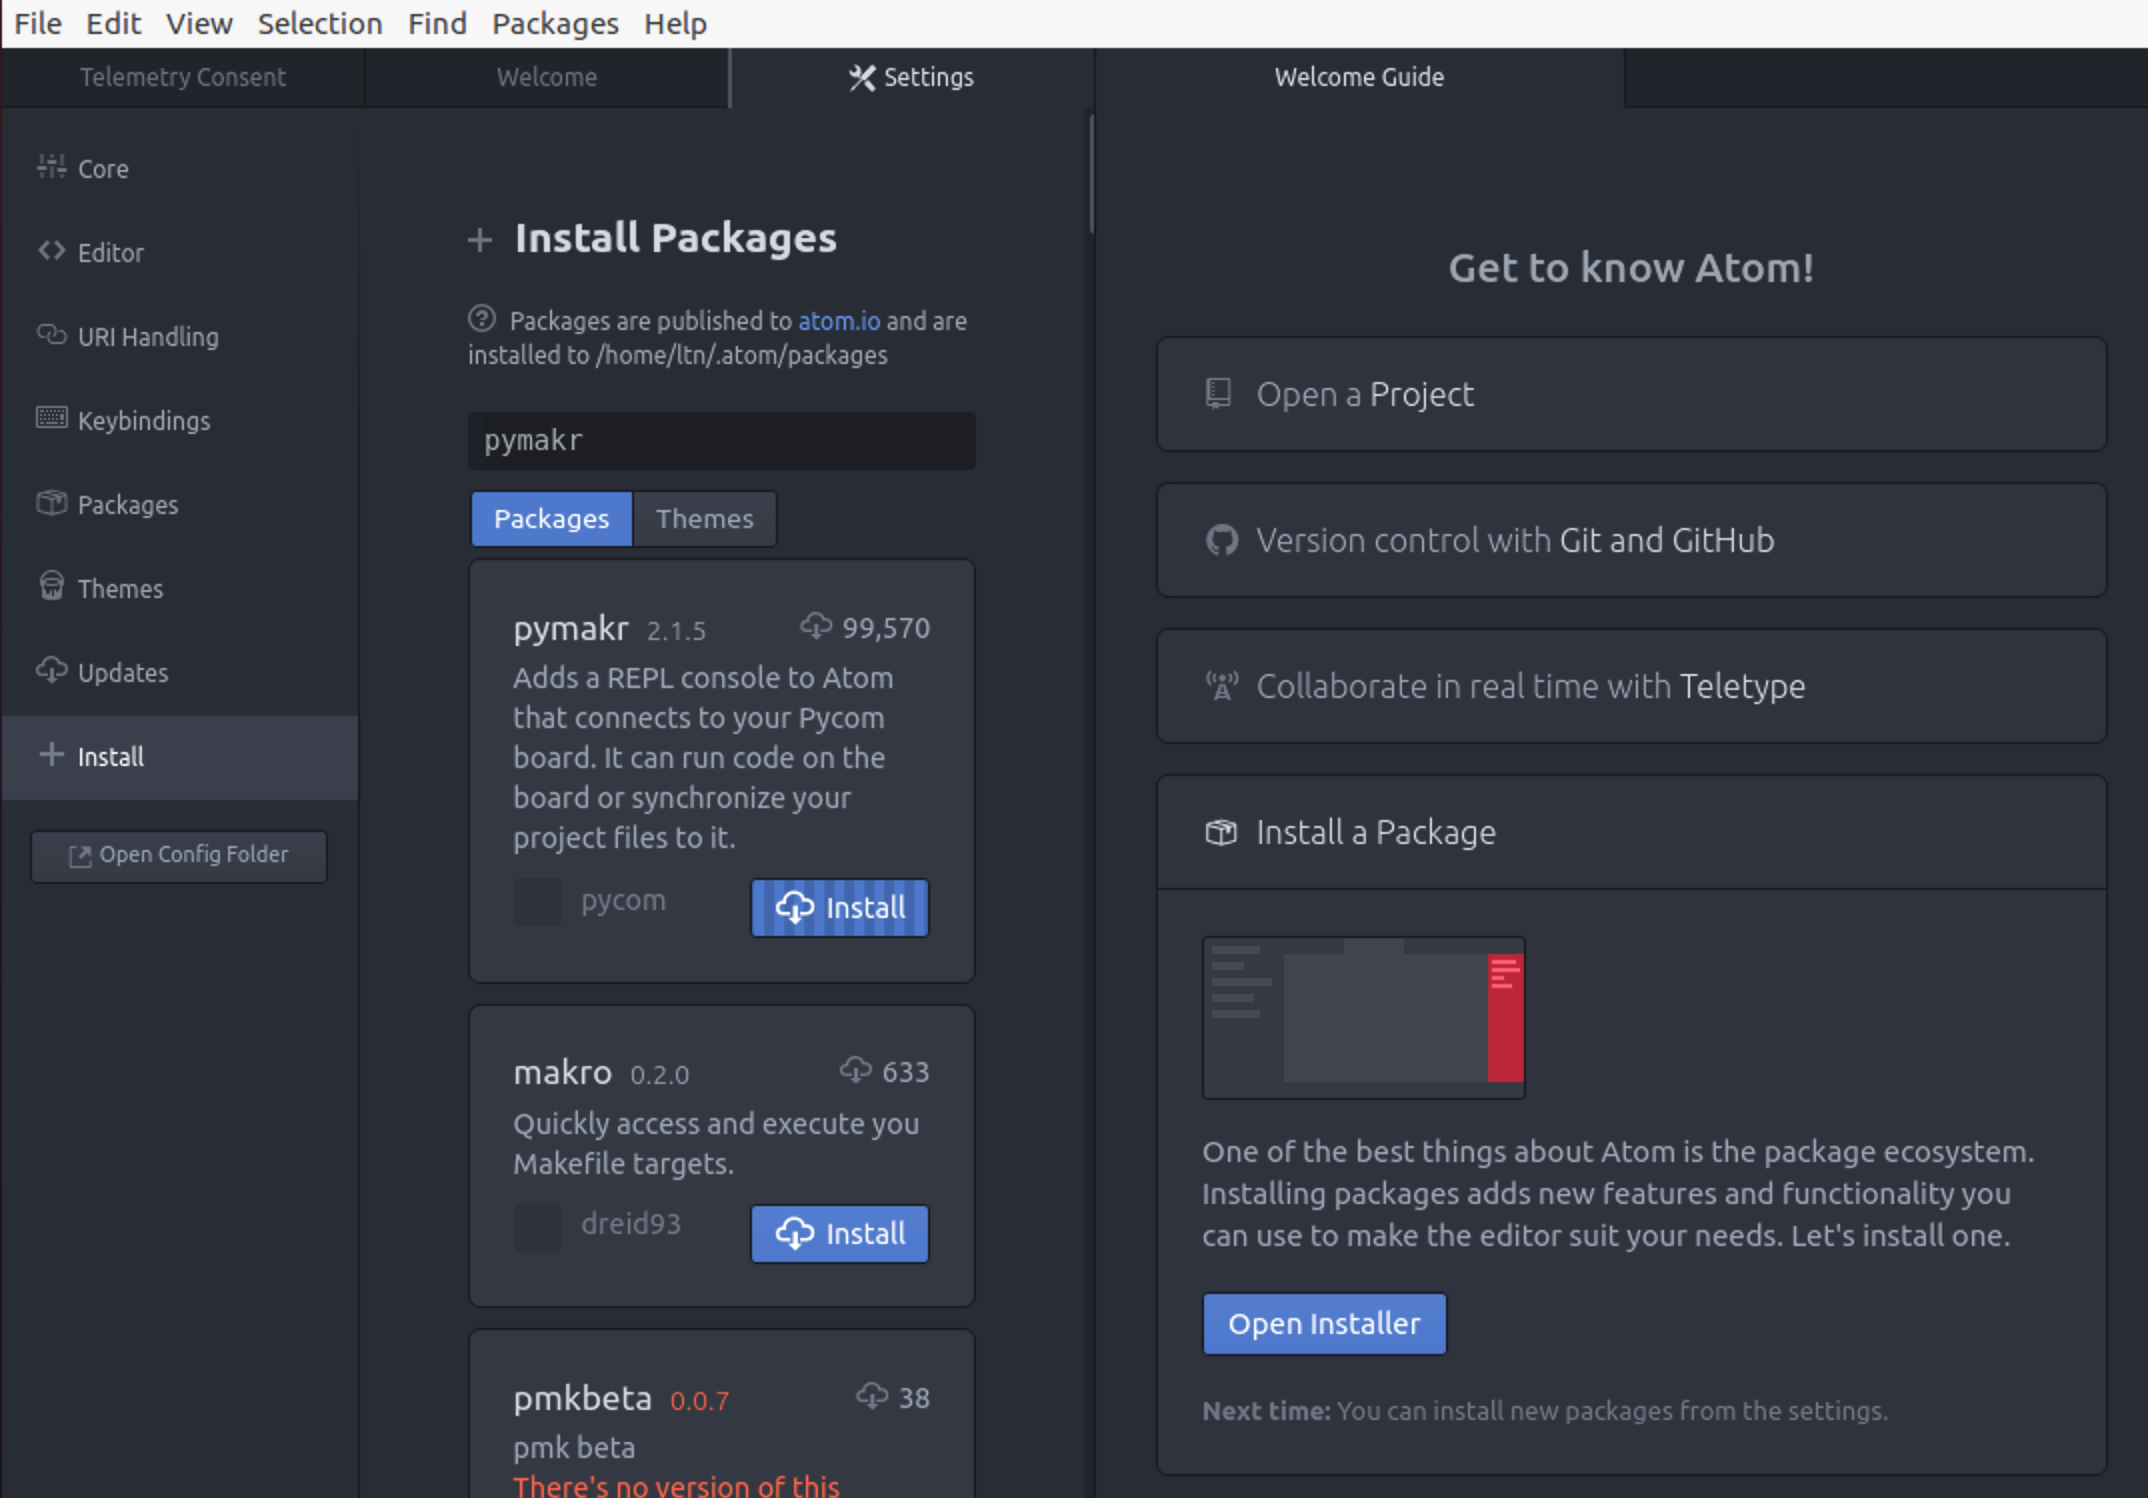
\includegraphics[width=1\columnwidth]{Pictures/atom_pymakr.png}}
\lgf{\caption{Installation de Paquetages}}
\lge{\caption{Package Installation}}
\label{fig-page-pakage}
\end{figure}

     \vspace{1em}

\lgf{Une fois le café bu et l’installation terminée, une nouvelle fenêtre (terminal) s’ouvre en bas d’Atom.}
\lge{Once the coffee is drunk and the installation is finished, a new window (terminal) opens at the bottom of Atom.}

     \vspace{1em}

\lgf{Ce terminal (cf.figure~\vref{fig-page-pymakr}) vous permettra de dialoguer avec le LoPy.
Branchez le LoPy à votre ordinateur.
Vous devriez voir l’invite\texttt{ >{}>{}>{}} caractéristique d’un interpréteur Python\footnote{Sous Linux, vous devez être membre du groupe dialout pour pouvoir gérer la communication sur le port USB. 
Si vous ne voyez par l’invite, tapez \texttt{sudo adduser \textit{login} dialout} en remplaçant login par le nom de votre compte Linux. Reconnectez-vous sous votre compte.}.}
\lge{This terminal (cf.figure~\vref{fig-page-pymakr}) will allow you to dialogue with the LoPy.
Connect the LoPy to your computer.
You should see the typical Python interpreter prompt \texttt{>{}>{}>{}}\footnote{Under Linux, you must be a member of the dialout group to be able to manage the communication on the USB port. 
If you do not see the prompt, type \texttt{sudo adduser \textit{login} dialout} replacing login with the name of your Linux account. Reconnect under your account}.}


     \vspace{1em}

\begin{figure}[tbp]
\centerline{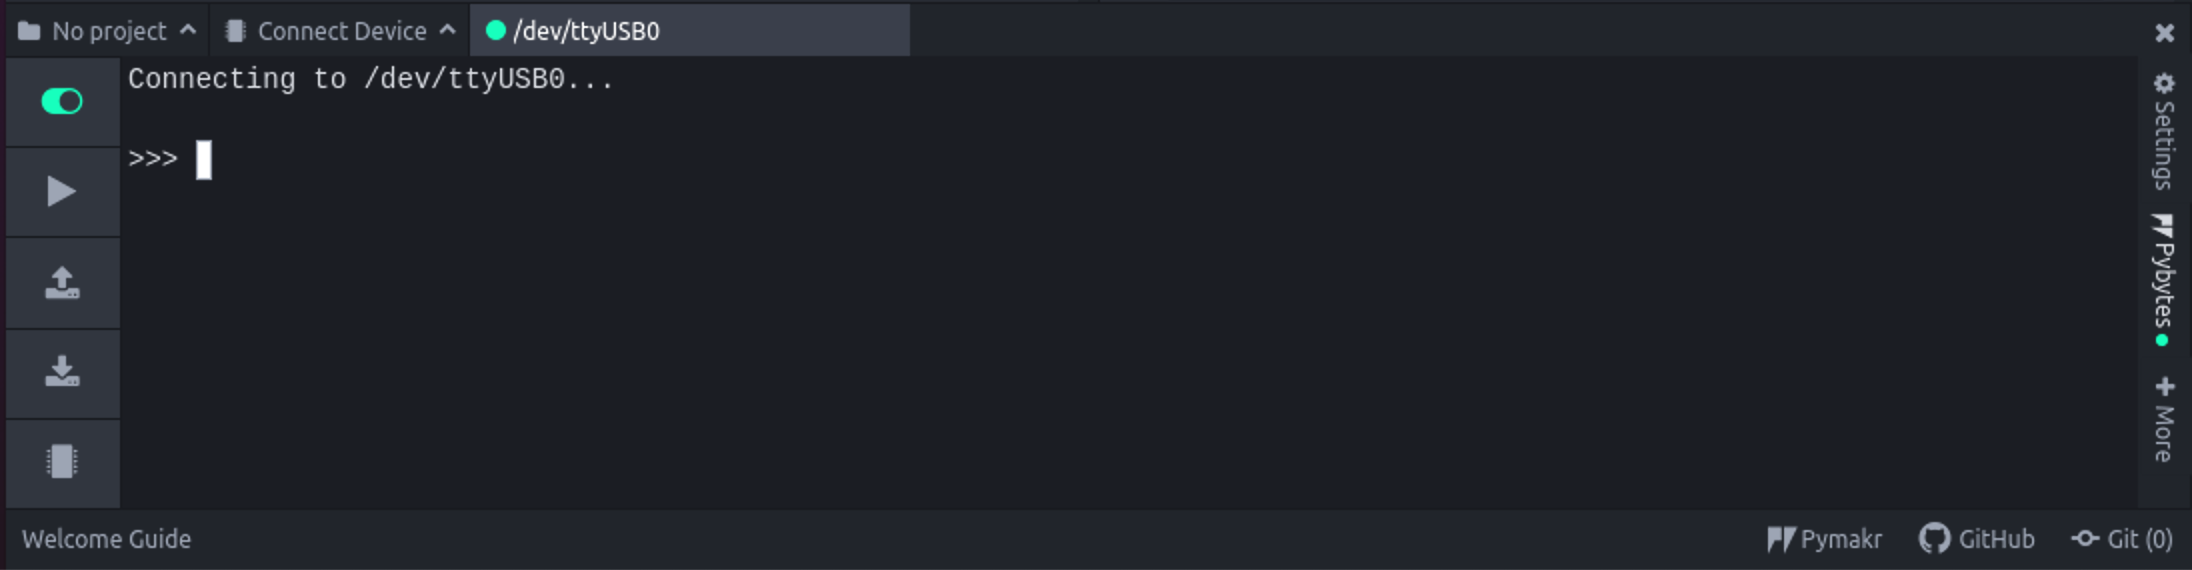
\includegraphics[width=1\columnwidth]{Pictures/atom_pymakr1.png}}
\lgf{\caption{Fenêtre Pymakr}}
\lge{\caption{Pymakr window}}
\label{fig-page-pymakr}
\end{figure}

\lgf{Toutes les commandes que vous allez taper dans cette fenêtre vont s’exécuter sur votre LoPy. Par exemple, si vous tapez\footnote{Les fenêtres sur fond gris montrent le code micropython et leur résultat.}~:}
\lge{All the commands you type in this window will run on your LoPy. For example, if you type \footnote{The windows with gray background show the micropython code and their result.}:}

\begin{termc}[backgroundcolor=\color{gray!10}, basicstyle=\ttfamily\small, escapechar=@]
Connecting to /dev/ttyUSB0...
>>> @\textbf{1+1}@
2
>>>
\end{termc}

\noindent
\lgf{l’addition se fait sur le LoPy.}
\lge{the addition is done on the LoPy.}


     \vspace{1em}

\lgf{Sur le coté gauche de la fenêtre pymakr, plusieurs icônes sont présentes~:}
\lge{On the left side of the pymakr window, several icons are present:}

\begin{itemize}
    \item 
        \lgf{l'interrupteur permet d'activer ou de désactiver le connexion avec le LoPy~;}
        \lge{the switch allows to activate or deactivate the connection with the LoPy;}
    \item  
        \lgf{le triangle permet d'exécuter le programme affiché dans la fenêtre d'Atom sur le LoPy~;}
        \lge{the triangle allows you to execute the program displayed in the Atom window on the LoPy;}
    \item  
        \lgf{la flèche vers le haut, permet de recopier le répertoire actif dans la mémoire du LoPy. Cela sera utile pour installer de nouveaux modules sur le LoPy~;}
        \lge{the up arrow, allows you to copy the active directory into the LoPy memory. This will be useful to install new modules on the LoPy;}
    \item  
        \lgf{inversement le flèche vers le bas, permet de recopier la mémoire du LoPy sur l'ordinateur~;}
        \lge{Conversely, the down arrow allows you to copy the memory of the LoPy to the computer;}
    \item  
        \lgf{le processeur permet d'avoir des informations sur le loPy.}
        \lge{the processor allows to have information about the loPy.}
\end{itemize}

     \vspace{1em}

\lgf{Sur la partie droite, l'onglet vertical \textit{Setting} permet de modifier les paramètres de connexion avec le LoPy.}
\lge{On the right side, the vertical tab \textit{Setting} allows to modify the connection parameters with the LoPy.}


\lgf{\subsection{Installez votre environnement de travail} }
\lge{\subsection{Set up your work environment} }

\lgf{Pour programmer le LoPy, il faut récupérer les modules micropython. Le dépôt ca être téléchargé dans le répertoire de votre choix~:}
\lge{To program the LoPy, you have to get the micropython modules. The repository can be downloaded in the directory of your choice:}


\begin{termc}[backgroundcolor=\color{gray!10},  basicstyle=\ttfamily\small, escapechar=@]
> git clone https://github.com/ltn22/PLIDObis.git
\end{termc}

\lgf{Dans le menu \textit{Files>Open Folder} d’Atom, sélectionnez le répertoire \texttt{pycom} du dépot téléchargé, et validez. Sur la partie gauche de l’écran, l’ensemble des fichiers composant ce répertoire apparaissent. Il y en a beaucoup, car ils vont nous servir par la suite.}
\lge{In Atom's \textit{Files>Open Folder} menu, select the \texttt{pycom} directory of the downloaded repository, and validate. On the left side of the screen, all the files composing this directory appear. There are a lot of them, because they will be used later.}


     \vspace{1em}

\lgf{En cliquant dans la fenêtre \textit{\Index{pymakr}} sur le bouton \textit{Upload project to device}, les fichiers de ce répertoire vont être copiés dans la mémoire du LoPy. 
Par la suite, si un module est modifié, il devra être resynchronisé dans la mémoire du LoPy.}
\lge{By clicking in the window \textit{Index{pymakr}} on the button \textit{Upload project to device}, the files of this directory will be copied in the memory of LoPy. 
Afterwards, if a module is modified, it will have to be resynchronized in the memory of LoPy.}

\lgf{\section{Connexion au réseau Wi-Fi}}
\lge{\section{Connection to the Wi-Fi network}}


\begin{wrapfigure}{r}{3cm}
\Youtube{https://youtu.be/PmvSU8AWO68}
\end{wrapfigure}


\lgf{Pour rattacher de LoPY à un réseau \Index{Wi-Fi}, il doit dans un premier temps être configuré via la liaison USB de l'ordinateur pour lui donner les paramètres nécessaires à la connexion. }
\lge{To attach LoPY to a \Index{Wi-Fi} network, it must first be configured via the USB link of the computer to give it the necessary parameters for the connection. }

\lgf{Le fichier \texttt{\Index{boot.py}} a été copié lors du téléversement des fichiers dans la mémoire du LoPy. Au démarrage du LoPy, ce programme va chercher à se connecte à un réseau Wi-Fi. Comme le nom du réseau et la clé sécrète n'ont pas été founie, il n’y arrive pas. Le LoPy se transforme  en point d’accès. Au démarrage, le LoPy a dû afficher le message suivant, indiquant que le LoPy devient point d'accès Wi-Fi et va déployer son propre réseau sur lequel votre ordinateur peut se connecter. Le nom de ce réseau de les la forme \texttt{PLIDO\_XXXX} où \texttt{XXXX} est une séquence hexadécimal propre à l'équipement. La clé est \texttt{www.pycom.io}. Le LoPy à l'adresse \texttt{192.168.4.1} sur ce réseau.  }
\lge{The file \texttt{Index{boot.py}} has been copied when uploading the files in the LoPy memory. When LoPy starts, this program will try to connect to a Wi-Fi network. As the network name and the secret key have not been provided, it does not succeed. The LoPy turns into an access point. At startup, the LoPy should have displayed the following message, indicating that the LoPy becomes a Wi-Fi access point and will deploy its own network on which your computer can connect. The name of this network has the form \texttt{PLIDO\_XXXX} where \texttt{XXXX} is a hexadecimal sequence specific to the equipment. The key is \texttt{www.pycom.io}. The LoPy at address \texttt{192.168.4.1} on this network.  }


\begin{termc}[backgroundcolor=\color{gray!10},  basicstyle=\ttfamily\small, escapechar=@]
Failed to connect to any known network, going into AP mode
To connect look for 'PLIDO_5bac' access point, key = 'www.pycom.io'
\end{termc}

\lgf{Mais ce n'est pas très intéressant car votre ordinateur va perdre sa connexion à l'internet. Pas très pratique pour suivre le MOOC. Avant d'afficher ce message, le LopY a montré la liste des réseaux Wi-Fi qu'il a détecté. Vous pouvez à l'inverse le connecter à un de ces réseau en renseignant le fichier \texttt{wifi\_conf.py} qui se trouve dans le répertoire \texttt{pycom}.}
\lge{But this is not very interesting because your computer will lose its connection to the internet. Not very practical to follow the MOOC. Before displaying this message, the LopY showed the list of Wi-Fi networks it detected. You can connect it to one of these networks by filling in the file \texttt{wifi\_conf.py} which is in the directory \texttt{pycom}.}

\pycomlst{wifi\_conf.py}

\lgf{\texttt{MON\_SSID} doit être remplacé par le nom du réseau Wi-Fi ou \ac{SSID} et \texttt{MON\_MOT\_DE\_PASSE} par la clé qui y est associée. Notez que plusieurs réseaux Wi-Fi peuvent être ajouté, puisque \texttt{MON\_SSID} est vu comme une clé de l'objet JSON. L'édition de fichier s'est faite sur l'ordinateur, il doit être recopié dans la mémoire du LoPy en cliquant sur la flèche vers le haut.}
\lge{\texttt{MON\_SSID} must be replaced by the name of the Wi-Fi network or \ac{SSID} and \texttt{MON\_MOT\_DE\_PASSE} by the key associated with it. Note that several Wi-Fi networks can be added, since \texttt{MON\_SSID} is seen as a key of the JSON object. The file edition was done on the computer, it must be copied in the memory of the LoPy by clicking on the up arrow.}

\lgf{Le Pycom redémarre et doit maintenant afficher un message du genre :}
\lge{The Pycom restarts and should now display a message like:}


\begin{termc}[backgroundcolor=\color{gray!10}, basicstyle=\ttfamily\small, escapechar=@]
net to use ['MONWIFI']
Connected to MONWIFI with IP address: @\ul{192.168.1.76}@
Pycom MicroPython 1.20.2.r1 [v1.11-a5aa0b8] on 2020-09-09; LoPy4 with ESP32
Type "help()" for more information.
>>> 
\end{termc}

\lgf{Il est possible de pinguer ou de se connecter avec \Index{FTP} ou \Index{telnet} en utilisant cette adresse IP.}
\lge{It is possible to ping or connect with \Index{FTP} or \Index{telnet} using this IP address.}

\begin{termc}[backgroundcolor=\color{palerod},  basicstyle=\ttfamily\small, escapechar=@]
# @\textbf{telnet \ul{192.168.1.76}}@
Trying 192.168.1.86...
Connected to 192.168.1.86.
Escape character is '^]'.
MicroPython v1.8.6-760-g90b72952 on 2017-09-01; LoPy with ESP32
Login as: micro
Password: python
Login succeeded!
Type "help()" for more information.
>>>
\end{termc}

\lgf{Ça peut être utile pour suivre le comportement de votre objet sans lancer atom si l'objet n'est plus connecté via la liaison USB à l'ordinateur. }
\lge{It can be useful to follow the behavior of your object without launching atom if the object is not connected via the USB link to the computer. }

\lgf{Atom peut également être configuré pour utiliser cette adresse IP. La configuration se fait dans le menu \textit{setting}, et en entrant l'adresse ip du LoPy et en désactivant \textit{auto connect}. Au prochain lancement d'Atom, il sera possible joindre le LoPy en Wi-Fi.}
\lge{Atom can also be configured to use this IP address. The configuration is done in the menu \textit{setting}, and by entering the ip address of the LoPy and disabling \textit{auto connect}. The next time Atom is launched, it will be possible to join the LoPy in Wi-Fi.}



\lgf{\section{Mise en place d'un client}}
\lge{\section{Setting up a client}}


\begin{wrapfigure}{r}{3cm}
\Youtube{https://youtu.be/Mi3e4c2E59o}
\end{wrapfigure}


\lgf{Un programme relativement simple permet de vérifier la communication entre le LoPy et le serveur. La commande \Index{ifconfig}\footnote{Sous Linux, il faut ajouter le paquetage \Index{net-tools} \texttt{sudo apt install net-tools}.} donne l'adresse IP du serveur. L'adresse doit être différente de celle que l'on avait obtenu sur le LoPy. }
\lge{A relatively simple program allows to check the communication between the LoPy and the server. The command \Index{ifconfig}\footnote{Under Linux, it is necessary to add the package \Index{net-tools} \texttt{sudo apt install net-tools}.} gives the server IP address. The address must be different from the one we had obtained on the LoPy. }

\lgf{Si le serveur tourne dans un environnement local, l'adresse devrait commencer par \texttt{192.168} ou \texttt{10}. Si le LoPy et l'ordinateur sont connectés au même réseau Wi-Fi, les premiers chiffres doivent être identiques. }
\lge{If the server is running in a local environment, the address should start with \texttt{192.168} or \texttt{10}. If the LoPy and the computer are connected to the same Wi-Fi network, the first digits must be identical. }

\lgf{Si le serveur tourne sur un serveur à l'extérieur (i.e. le \textit{cloud}), l'adresse est quelconque.}
\lge{If the server is running on an external server (i.e. the \textit{cloud}), the address is random.}

     \vspace{1em}

\lgf{La commande suivante est tapée depuis le terminal de l'ordinateur, on remarque les deux interfaces disponibles l'une pour le réseau Ethernet ou Wi-Fi et l'une pour le \textit{\Index{loopback}}, les noms des interfaces peuvent changer d'une configuration à une autre~:}
\lge{The following command is typed from the terminal of the computer, we notice the two available interfaces one for the Ethernet or Wi-Fi network and one for the \textit{\Index{loopback}}, the names of the interfaces can change from one configuration to another:}

\begin{termc}[backgroundcolor=\color{palerod},  basicstyle=\ttfamily\small, escapechar=@]
> @\textbf{ifconfig}@
eth1      Link encap:Ethernet  HWaddr 10:65:30:b0:54:bf
          inet addr:@\ul{192.168.1.237}@  Bcast:192.168.1.255  Mask:255.255.255.0
          inet6 addr: fe80::d8ac:86e7:8bdb:e333/64 Scope:Unknown
          UP BROADCAST RUNNING MULTICAST  MTU:1500  Metric:1
          RX packets:0 errors:0 dropped:0 overruns:0 frame:0
          TX packets:0 errors:0 dropped:0 overruns:0 carrier:0
          collisions:0
          RX bytes:0 (0.0 B)  TX bytes:0 (0.0 B)

lo        Link encap:Local Loopback
          inet addr:127.0.0.1  Mask:255.0.0.0
          inet6 addr: ::1/128 Scope:Unknown
          UP LOOPBACK RUNNING  MTU:1500  Metric:1
          RX packets:0 errors:0 dropped:0 overruns:0 frame:0
          TX packets:0 errors:0 dropped:0 overruns:0 carrier:0
          collisions:0
          RX bytes:0 (0.0 B)  TX bytes:0 (0.0 B)
\end{termc}

\lgf{Le programme \pprog{minimal\_server.py}{plido-tp3} présenté au chapitre~\vref{chap-mini-serv} n'a pas été modifié et attend des données sur le port 33033.}
\lge{The program \pprog{minimal\_server.py}{plido-tp3} presented in chapter~\vref{chap-mini-serv} has not been modified and waits for data on port 33033.}


     \vspace{1em}

\pycomlst{sending\_client.py}

\lgf{Le programme \lprog{sending\_client.py}{pycom} doit être modifié (ligne 4) pour prendre en compte l'adresse IP du serveur obtenue avec la commande \texttt{ifconfig}. Si à chaque exécution sur le LoPy de ce programme, le serveur reçoit la valeur, la communication est établie entre les deux équipements.}
\lge{The program \lprog{sending\_client.py}{pycom} must be modified (line 4) to take into account the IP address of the server obtained with the command \texttt{ifconfig}. If at each execution on the LoPy of this program, the server receives the value, the communication is established between the two devices.}


\begin{termc}[backgroundcolor=\color{palerod}, basicstyle=\ttfamily\small, escapechar=@]
> @\textbf{python3 minimal\_server.py}@
b'message' => b'6d657373616765'
b'message' => b'6d657373616765'
\end{termc}


\section{BME 280}

\begin{wrapfigure}{r}{3cm}
\Youtube{https://youtu.be/I3zc3-qoq2s}
\end{wrapfigure}

\lgf{Au lieu de générer de fausses données, nous allons dans cette section utiliser un vrai capteur de température humidité pression : le BME 280 de chez Bosch. }
\lge{Instead of generating false data, we will use in this section a real temperature humidity pressure sensor: the BME 280 from Bosch. }


\lgf{\subsection{Le bus I2C}}
\lge{\subsection{I2C bus}}


\lgf{Le bus I2C est  normalisé par le fabricant de composants électroniques  \Index{NXP}\footnote{\url{https://www.nxp.com/docs/en/user-guide/UM10204.pdf}} ce qui permet une meilleure interopérabilité entre les composants.}
\lge{The I2C bus is standardized by the electronic components manufacturer \Index{NXP}\footnote{url{https://www.nxp.com/docs/en/user-guide/UM10204.pdf}} which allows a better interoperability between the components.}


 \begin{figure}[!ht] 
\centering 


	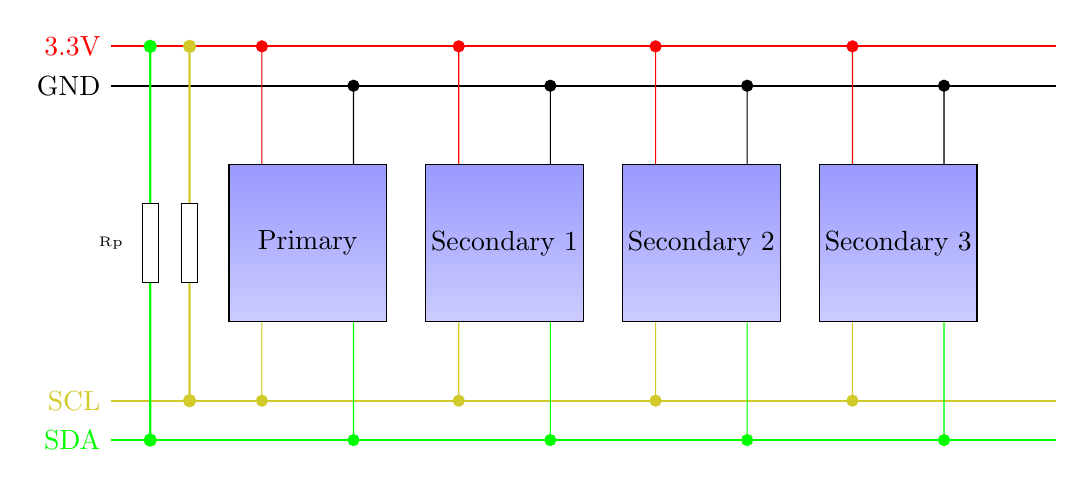
\begin{tikzpicture}
	
	\draw [thick, red] (0, 7.5) node [left] {3.3V} coordinate (l1) -- +(12, 0); 
	\draw [thick, black] (0, 7) node [left] {GND} coordinate (l2) -- +(12, 0); 
	
	\draw [thick, yellow!80!black] (0, 3) node [left] {SCL} coordinate (l3) -- +(12, 0); 
	\draw [thick, green] (0, 2.5) node [left] {SDA} coordinate (l4) -- +(12, 0); 
	
	\foreach \i/\n in {1/Primary, 2/Secondary 1, 3/Secondary 2, 4/Secondary 3} {
		\draw (2.5*\i, 5) node (n\i) [rectangle, top color=blue!40, bottom color=blue!20, draw, minimum size= 2cm]{};
		
		\draw (n\i) node {\n};
		
		\filldraw [red] (n\i.120) -- (n\i.120 |-l1) circle  (2pt);
		\filldraw [black] (n\i.60) -- (n\i.60 |-l2) circle  (2pt);
		\filldraw [yellow!80!black] (n\i.-120) -- (n\i.-120 |-l3) circle  (2pt);
		\filldraw [green] (n\i.-60) -- (n\i.-60 |-l4) circle  (2pt);
	}

	\coordinate (v1) at (0.5, 0);
	\coordinate (v2) at (1, 0);
	
	\filldraw [thick, green] (v1 |- l1) circle  (2pt) -- coordinate (r1) (v1 |- l4)circle  (2pt);
	\filldraw [thick, yellow!80!black] (v2 |- l1)circle  (2pt) -- coordinate (r2) (v2 |- l3)circle  (2pt);
	
	\filldraw [white]  ([xshift=-0.1cm, yshift=-0.5cm]r1) rectangle ++(0.2, 1); 
	\draw ([xshift=-0.1cm, yshift=-0.5cm]r1) rectangle ++(0.2, 1); 
	
	\draw  ([xshift=-0.5cm]r1) node {\tiny{Rp}};
	
	\filldraw [white] ([xshift=-0.1cm, yshift=-0.5cm]r1-|r2) rectangle ++(0.2, 1); 
	\draw ([xshift=-0.1cm, yshift=-0.5cm]r1-|r2) rectangle ++(0.2, 1); 
	
	

	\end{tikzpicture}
\lgf{\caption{bus I2C} }
\lge{\caption{I2C bus} }

\label{fig-busI2C} 
\end{figure} 	

\lgf{Sur un des fils le signal d'horloge va être émis par le primaire. Sur l'autre fil, les données seront codées soit dans le sens primaire/secondaire, soit dans l'autre. Comme avec \Index{Modbus}, les communications entre un secondaire et le primaire seront gérées par le primaire. 
Chaque secondaire est configuré avec une adresse unique sur le bus. Soit le maître envoie des données vers cette adresse\footnote{Il s'agit d'un abus de langage, en effet les données émises par le primaire sont reçues par l'ensemble des secondaires, mais seul celui qui est destinataire (i.e. qui reconnaît son adresse) va les traiter, les autres équipements ignoreront l'information.}, soit le primaire interroge l'esclave pour obtenir ses données. Le fil sera donc exploité dans les deux directions. }
\lge{On one of the wires the clock signal will be transmitted by the primary. On the other wire, the data will be coded either in the primary/secondary direction, or in the other. As with \Index{Modbus}, the communications between a secondary and the primary will be managed by the primary. 
Each secondary is configured with a unique address on the bus. Either the master sends data to this address, or the primary interrogates the slave to obtain its data. The wire will thus be exploited in both directions. }


\lgf{La lecture de l'information binaire se fait lorsque le signal d'horloge est à l'état haut (cf. figure~\vref{fig-exI2C}). Quand le signal SDA est à l'état haut, un bit à 1 est transmis et dans l'état bas un bit à 0 est transmis.  Les changements d'état du signal SDA se font donc quand le signal d'horloge est à l'état bas. }
\lge{The reading of the binary information is done when the clock signal is in the high state (see figure~\vref{fig-exI2C}). When the SDA signal is in the high state, a 1 bit is transmitted and in the low state a 0 bit is transmitted.  The changes of state of the SDA signal are thus done when the clock signal is in the low state. }

\lgf{Il existe malgré tout deux exceptions~: si le signal SDA passe de l'état haut à l'état bas tandis que le signal d'horloge est à l'état haut cela indique un début de transmission de données. Si le signal SDA passe de l'état bas à l'état haut dans les mêmes conditions, cela indique la fin de transmission de données. Entre les deux les données binaires forment une trame (ou un PDU dans le vocabulaire ISO) qui est structuré comme indiqué figure~\vref{fig-exI2C}.}
\lge{However, there are two exceptions: if the DID signal goes from high to low while the clock signal is high, this indicates the start of data transmission. If the DID signal goes from low to high under the same conditions, this indicates the end of data transmission. Between the two the binary data form a frame (or PDU in ISO vocabulary) which is structured as shown in figure~\vref{fig-exI2C}.}

  \begin{figure}[!ht] 
\centering 
 \pgfdeclarelayer{foreground}
 \pgfdeclarelayer{background}

\begin{tikztimingtable} [timing/d/background/.style={fill=white}, timing/lslope=0.2]
            SDA & H H L L L 4D 4D; [dotted] 4D; 4D 4D  LLLL HHHH\\
            SCL & HHHH 2T 2T 2T 2T 2T; [dotted] 2T; 2T 2T 2T 2T 2T HHHHHH \\
 \extracode
 % Add vertical lines in two colors
  \begin{pgfonlayer}{background}
    \begin{scope}[semitransparent,semithick]
      \draw   (2.2, 1.2) node (S) [below, rectangle, draw, minimum width=0.4cm,minimum height=1.2cm, pattern=dots, pattern color=purple]{};
      \draw (S.south) node [below] {S};
      
      \draw   (29, 1.2) node (P) [below, rectangle, draw, minimum width=0.4cm,minimum height=1.2cm, pattern=dots, pattern color=purple]{};
      \draw (P.south) node [below] {P};
      
     \foreach \i in {7.1,11.1,...,23.1} {
       \draw   (\i, 1.2) node (B) [below, rectangle, draw, minimum width=0.4cm,minimum height=1.2cm, color=purple]{};
        \draw (B.south) node [below] {0/1};
  
     }
    \end{scope}
  \end{pgfonlayer}
 
 \end{tikztimingtable}%

\lgf{\caption{Exemple de communication avec le bus I2C} }
\lge{\caption{Example of communication with the I2C bus} }

\label{fig-exI2C} 
\end{figure}

\lgf{La figure~\vref{fig-tramesI2C} donne les formats les plus utilisés. }
\lge{Figure~\vref{fig-framesI2C} gives the most used formats. }


\begin{figure}[!ht] 
\centering 
\begin{tikzpicture}

	\draw (0,0) node (S) [rectangle, draw, pattern=dots, pattern color=purple, minimum width=0.3cm, minimum height=0.5cm]{};
	\draw (S) node {\tiny{S}};  
	
	\coordinate (a) at (S.east);
	\foreach \i in {7,...,1}{
 		\draw (a) node (A\i) [right, rectangle, draw, fill=purple, minimum width=0.3cm, minimum height=0.5cm]{};
 		\draw (A\i) node [text width=0.3cm, text centered] {\tiny{A\\\i\\}};
 		
 		\coordinate (a) at (A\i.east);	
	}
 	\draw (a) node (RW) [right, rectangle, draw, fill=purple, minimum width=0.3cm, minimum height=0.5cm]{};
 	\draw (RW) node [text width=0.3cm, text centered] {\tiny{0\\}};


 	\draw (RW.east) node (Ack1) [right, rectangle, draw, fill=yellow, minimum width=0.3cm, minimum height=0.5cm]{};
 	\draw (Ack1) node [text width=0.3cm, text centered] {\fontsize{6}{4}{\selectfont a\\c\\k\\}};
 	
 	\coordinate (a) at (Ack1.east);
	\foreach \i in {8,...,1}{
 		\draw (a) node (D1-\i) [right, rectangle, draw, fill=purple, minimum width=0.3cm, minimum height=0.5cm]{};
 		\draw (D1-\i) node [text width=0.3cm, text centered] {\tiny{D\\\i\\}};
 		
 		\coordinate (a) at (D1-\i.east);	
	}
 	\draw (a) node (Ack2) [right, rectangle, draw, fill=yellow, minimum width=0.3cm, minimum height=0.5cm]{};
 	\draw (Ack2) node [text width=0.3cm, text centered] {\fontsize{6}{4}{\selectfont a\\c\\k\\}};

 	\draw [dashed] (Ack2) -- ++(1, 0) coordinate (a);
	\foreach \i in {8,...,1}{
 		\draw (a) node (D2-\i) [right, rectangle, draw, fill=purple, minimum width=0.3cm, minimum height=0.5cm]{};
 		\draw (D2-\i) node [text width=0.3cm, text centered] {\tiny{D\\\i\\}};
 		
 		\coordinate (a) at (D2-\i.east);	
	}
 	\draw (a) node (Ack3) [right, rectangle, draw, fill=yellow, minimum width=0.3cm, minimum height=0.5cm]{};
 	\draw (Ack3) node [text width=0.3cm, text centered] {\fontsize{6}{4}{\selectfont a\\c\\k\\}};
	
	\draw (Ack3.east) node (P) [right, rectangle, draw, pattern=dots, pattern color=purple, minimum width=0.3cm, minimum height=0.5cm]{};
	\draw (P) node {\tiny{P}};  


	\draw (0,-1) node (S) [rectangle, draw, pattern=dots, pattern color=purple, minimum width=0.3cm, minimum height=0.5cm]{};
	\draw (S) node {\tiny{S}};  
	
	\coordinate (a) at (S.east);
	\foreach \i in {7,...,1}{
 		\draw (a) node (A\i) [right, rectangle, draw, fill=purple, minimum width=0.3cm, minimum height=0.5cm]{};
 		\draw (A\i) node [text width=0.3cm, text centered] {\tiny{A\\\i\\}};
 		
 		\coordinate (a) at (A\i.east);	
	}
 	\draw (a) node (RW) [right, rectangle, draw, fill=purple, minimum width=0.3cm, minimum height=0.5cm]{};
 	\draw (RW) node [text width=0.3cm, text centered] {\tiny{1\\}};


 	\draw (RW.east) node (Ack1) [right, rectangle, draw, fill=yellow, minimum width=0.3cm, minimum height=0.5cm]{};
 	\draw (Ack1) node [text width=0.3cm, text centered] {\fontsize{6}{4}{\selectfont a\\c\\k\\}};
 	
 	\coordinate (a) at (Ack1.east);
	\foreach \i in {8,...,1}{
 		\draw (a) node (D1-\i) [right, rectangle, draw, fill=yellow, minimum width=0.3cm, minimum height=0.5cm]{};
 		\draw (D1-\i) node [text width=0.3cm, text centered] {\tiny{D\\\i\\}};
 		
 		\coordinate (a) at (D1-\i.east);	
	}
 	\draw (a) node (Ack2) [right, rectangle, draw, fill=purple, minimum width=0.3cm, minimum height=0.5cm]{};
 	\draw (Ack2) node [text width=0.3cm, text centered] {\fontsize{6}{4}{\selectfont a\\c\\k\\}};
 	
 	\draw [dashed] (Ack2) -- ++(1, 0) coordinate (a);

	\foreach \i in {8,...,1}{
 		\draw (a) node (D2-\i) [right, rectangle, draw, fill=yellow, minimum width=0.3cm, minimum height=0.5cm]{};
 		\draw (D2-\i) node [text width=0.3cm, text centered] {\tiny{D\\\i\\}};
 		
 		\coordinate (a) at (D2-\i.east);	
	}
 	\draw (a) node (Ack3) [right, rectangle, draw, fill=purple, minimum width=0.3cm, minimum height=0.5cm]{};
 	\draw (Ack3) node [text width=0.3cm, text centered] {\fontsize{6}{4}{\selectfont a\\c\\k\\}};
	
	\draw (Ack3.east) node (P) [right, rectangle, draw, pattern=dots, pattern color=purple, minimum width=0.3cm, minimum height=0.5cm]{};
	\draw (P) node {\tiny{P}};  

\end{tikzpicture}


\lgf{\caption{Exemple de communication avec le bus I2C}}
\lge{\caption{Example of communication with the I2C bus}}

\label{fig-tramesI2C} 
\end{figure} 

\lgf{Le premier train binaire illustre la transmission de données du primaire vers un secondaire. Le primaire commence par émettre un signal non binaire (\texttt{S}) indiquant un début de transmission. Les 7 bits suivants donnent l'adresse du secondaire et le bit suivant indique si le primaire veut envoyer des données (valeur à \texttt{0}) ou recevoir des informations du secondaire (valeur à \texttt{1}). }
\lge{The first bit stream illustrates the transmission of data from the primary to a secondary. The primary starts by emitting a non-binary signal (\texttt{S}) indicating a start of transmission. The next 7 bits give the address of the secondary and the next bit indicates whether the primary wants to send data (value at \texttt{0}) or receive information from the secondary (value at \texttt{1}). }

\lgf{Si un secondaire reconnaît son adresse sur le bus, alors il écrit le bit suivant dans le train binaire. Le primaire est donc informé en lisant cette valeur que le secondaire est bien présent sur le bus et qu'il peut recevoir des données. Le primaire va donc les envoyer octet par octet. Chaque octet étant acquitté de la même manière par le secondaire. Le train binaire se termine par le signal non binaire (\texttt{P}).}
\lge{If a secondary recognizes its address on the bus, then it writes the next bit in the bitstream. The primary is thus informed by reading this value that the secondary is indeed present on the bus and that it can receive data. The primary will then send them byte by byte. Each byte is acknowledged in the same way by the secondary. The binary train ends with the non-binary signal (\texttt{P}).}

\lgf{Dans le cas où le primaire souhaite recevoir, une fois le bit de début et les bits de l'adresse émis, le huitième bit est positionné à 1. Le secondaire acquitte puis transmet ses octets que le primaire acquitte.}
\lge{In the case where the primary wishes to receive, once the start bit and the address bits have been transmitted, the eighth bit is set to 1. The secondary acknowledges and then transmits its bytes which the primary acknowledges.}


\Question{scan}
{
\lgf{Le module I2C du LoPy dispose d'une fonction \pfunction{machine}{scan} qui affiche les adresses des secondaires connectés. Comment cette détection est possible ?}
\lge{The I2C module of LoPy has a function \pfunction{machine}{scan} which displays the addresses of the connected secondaries. How is this detection possible?}
}
{
\lgf{Le primaire va tester toutes les adresses possibles et y envoyer une trame, si le bit suivant l'adresse dans la trame n'est pas positionné par le secondaire, il n'y a aucun équipement connecté à cette adresse.}
\lge{The primary will test all possible addresses and send a frame, if the bit following the address in the frame is not set by the secondary, there is no equipment connected to that address.}
}

\Question{\lgf{Diffusion}\lge{Broadcast}}
{
\lgf{Est-ce que la norme une adresse qui permet de parler à tous les secondaires en même temps ?}
\lge{Is the standard an address that allows you to talk to all the secondaries at the same time?}
}
{
\lgf{La norme prévoit un \textit{General Call} pour joindre tous les secondaires en utilisant l'adresse 0 (voir chapitre 3.1.12 du standard I2C).}
\lge{The standard provides for a General Call to reach all the secondaries using address 0 (see chapter 3.1.12 of the I2C standard).}
}

\lgf{\subsection {Mesure de la température}}
\lge{\subsection {Temperature measurement}}

\lgf{La communication entre le LoPy et le composant se fait via le bus \Index{I2C}. Il nous faut donc quatre fils pour le relier (cf. figure~\vref{fig-lopy-bme280-i2c}~: }
\lge{The communication between the LoPy and the component is done via the bus \Index{I2C}. So we need four wires to connect it (see figure~\vref{fig-lopy-bme280-i2c}~: }

\begin{itemize}
    \item 
        \lgf{la masse (\texttt{\Index{GND}}), }
        \lge{the ground (\texttt{\Index{GND}}), }
    \item  
        \lgf{une alimentation électrique de 3.3v (\texttt{\Index{VIN}}), }
        \lge{a 3.3v power supply (\texttt{\Index{VIN}}), }
    \item  
        \lgf{un fils pour l'horloge (\texttt{\Index{SCL}}) et }
        \lge{a wire for the clock (\texttt{\Index{SCL}}) et }
    \item  
        \lgf{un autre finalement pour les données (\texttt{\Index{SDA}}).}
        \lge{another one finally for the data (\texttt{\Index{SDA}}).}
\end{itemize} 

\begin{figure}[tbp]
\centerline{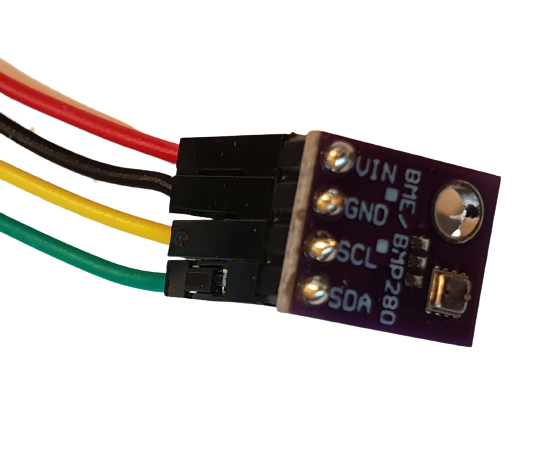
\includegraphics[width=.5\columnwidth]{Pictures/BME280-i2c.png}  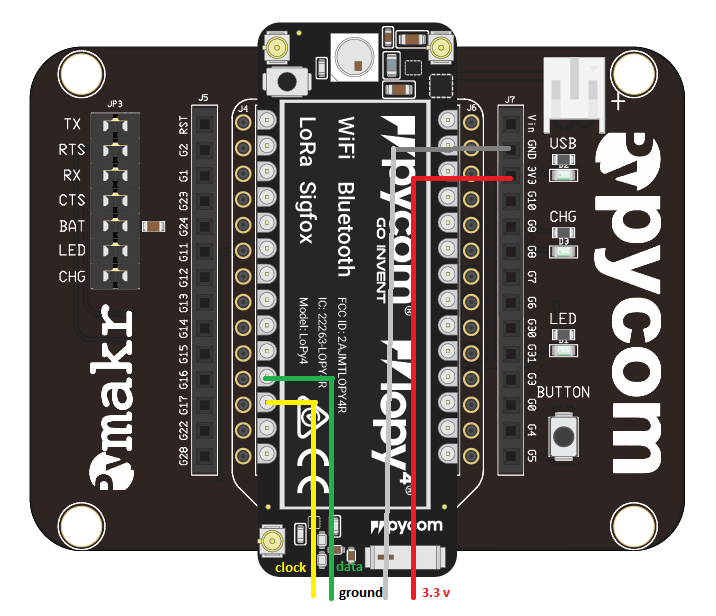
\includegraphics[width=.5\columnwidth]{Pictures/LoPy4.png}  }
\lgf{\caption{capteur BME280 et connecteurs}}
\lge{\caption{BME280 sensor and connectors}}
\label{fig-lopy-bme280-i2c}
\end{figure}

     \vspace{1em}

\lgf{Pour ce faire, il faut connecter~:}
\lge{To do this, you must connect:}
~\begin{itemize}
    \item   
        \lgf{la masse GND du LoPy sur la broche GND du composant avec un fil noir,}
        \lge{the GND of the LoPy to the GND pin of the component with a black wire,}
    \item   
        \lgf{l’alimentation en 3.3V du LoPy (3V3) sur VIN du composant avec un fil rouge (ce port s’appelle également \Index{DCC} sur certaines cartes),}
        \lge{3.3V power supply of LoPy (3V3) on VIN of the component with a red wire (this port is also called \Index{DCC} on some boards),}
    \item   
        \lgf{Le signal d’horloge du port G18/P10 du LoPy (ou G17 sur les versions LoPy 1) sur le port SCL du composant avec un fil jaune (ce port s’appelle également \Index{CLC} sur certaines cartes),}
        \lge{The clock signal from the G18/P10 port of LoPy (or G17 on LoPy 1 versions) on the SCL port of the component with a yellow wire (this port is also called \Index{CLC} on some boards),}
    \item   
        \lgf{Le fil de données du port G16/P9 du Pycom sur le port SDA du composant avec un fil vert.}
        \lge{The data wire from the Pycom G16/P9 port to the SDA port of the component with a green wire.}
\end{itemize}

\lgf{Si le BME280 est connecté correctement sur les connecteurs du LoPy, vous devez obtenir le résultat suivant~:}
\lge{If the BME280 is connected correctly to the LoPy connectors, you should get the following result:}

\begin{termc}[backgroundcolor=\color{gray!10}, basicstyle=\ttfamily\tiny, escapechar=@]
>>> Running BME280.py

>>> 
>>> 
[118]
temp 550576 27.98  - hum 26626 48.784 % - pres 389338 pres 1004.494 hPa [delta -389338 ]
temp 551952 28.42  - hum 26587 48.557 % - pres 389712 pres 1004.527 hPa [delta -374 ]
temp 551792 28.37  - hum 26577 48.491 % - pres 389664 pres 1004.621 hPa [delta 48 ]
temp 551712 28.34  - hum 26594 48.596 % - pres 389648 pres 1004.654 hPa [delta 16 ]
temp 551632 28.32  - hum 26587 48.546 % - pres 389616 pres 1004.713 hPa [delta 32 ]
\end{termc}

\lgf{Vous pouvez soit toucher le capteur, soit souffler dessus pour faire augmenter la température ou la pression.}
\lge{You can either touch the sensor or blow on it to increase the temperature or pressure.}

     \vspace{1em}

\pycomlst[firstline=282, firstnumber=282]{BME280.py} %[firstline=282,lastline=19, firstnumber=282]

\lgf{Le programme \lprog{BME280.py}{pycom} peut fonctionner comme un module mais la dernière partie donne un exemple d'exploiation des résultats~:}
\lge{The program \lprog{BME280.py}{pycom} can work as a module but the last part gives an example of exploitation of the results:}

\begin{itemize}

\item 
    \lgf{Le programme principal commence par importer (ligne 283) le module gérant le bus I2C. Il est invoqué à la ligne 286. Le LoPy va gérer la communication avec le BME280, donc l’adresse est \texttt{0} et son statut est\texttt{MASTER}. La vitesse de communication est ensuite spécifiée.}    
    \lge{The main program starts by importing (line 283) the module managing the I2C bus. It is invoked at line 286. The LoPy will manage the communication with the BME280, so the address is \texttt{0} and its status is \texttt{MASTER}. The communication speed is then specified.}

\item 
    \lgf{La ligne suivante scanne le bus pour trouver des composants. Si tout va bien, il devrait en trouver un à l’adresse 118 qui correspond à  l’adresse par défaut du BME280\footnote{Si une autre valeur est indiquée, vous pouvez à l'instantiation du module BME280, ligne 289, ajouter le paramètre \texttt{addr=\textit{valeur}}. }. Sinon, revoyez votre câblage.}
    \lge{The next line scans the bus for components. If all goes well, it should find one at address 118, which is the default address of the BME280. \footnote{If another value is indicated, you can add the parameter \texttt{addr=\textit{value}} to the instantiation of the BME280 module, line 289. }. Otherwise, review your wiring.}

\item 
    \lgf{Le module BME280 est initialisé en lui passant en paramètre la référence du bus I2C précédemment défini.}
    \lge{The BME280 module is initialized by passing the previously defined I2C bus reference as a parameter.}

\item 
    \lgf{Le programme va ensuite afficher les valeurs captées par le composant. Il existe deux types de valeurs : brutes (\textit{raw}) et calibrées. Les premières réagissent plus rapidement aux changements cependant sont beaucoup plus bruitées que les secondes qui subissent un traitement mathématique.}
    \lge{The program will then display the values captured by the component. There are two types of values: raw (\textit{raw}) and calibrated. The first ones react more quickly to changes but are much noisier than the second ones which undergo a mathematical processing.}

    \lgf{Ainsi, les première et deuxième colonnes donnent les températures brute et calibrée. On y accède par les méthodes \pfunction{BME280}{read\_raw\_temp} et \pfunction{BME280}{read\_temperature}. Il en va de même pour les deux autres grandeurs, humidité et pression.}
    \lge{Thus, the first and second columns give the raw and calibrated temperatures. They are accessed by the methods \pfunction{BME280}{read\_raw\_temp} and \pfunction{BME280}{read\_temperature}. It is the same for the two other quantities, humidity and pressure.}
\item 
    \lgf{Le programme affiche également l’écart de pression brute entre deux mesures. Cela permet de mettre plus facilement en évidence le fait que l’on souffle sur le capteur.}
    \lge{The program also displays the raw pressure difference between two measurements. This makes it easier to highlight the fact that the sensor is being blown.}
\end{itemize}

\lgf{\section{Thermomètre Wi-Fi}}
\lge{\section{Wi-Fi thermometer}}

\begin{wrapfigure}{r}{3cm}
\Youtube{https://youtu.be/Ie-hGkkhsMQ}
\end{wrapfigure}

\lgf{Vous avez maintenant tous les outils pour récupérer la température de votre logement, la transmettre à votre ordinateur via le Wi-Fi, et la transmettre à Beebotte pour l'afficher. Il y a très peu de changement par rapport à la version complètement sur ordinateur. Le programme de transformation de la structure CBOR de représentation des séries temporelles en JSON compréhensible par Beebottte reste le même. Il faudra juste modifier le nom du capteur d'humidité à température.}
\lge{You now have all the tools to retrieve the temperature of your home, transmit it to your computer via Wi-Fi, and transmit it to Beebotte for display. There is very little change from the fully computerized version. The program to transform the CBOR structure of the time series representation into JSON understandable by Beebottte remains the same. It will just be necessary to modify the name of the humidity to temperature sensor.}

\lgf{Le programme que vous avez construit lors du TP précédent utilisait le module \texttt{virtual\_sensor} pour produire des séries temporelles aléatoires symbolisant le comportement d'un capteur. Maintenant que nous avons un \Index{BME280}, nous allons pouvoir traiter de vraies valeurs.}
\lge{The program you built in the previous tutorial used the module \texttt{virtual\_sensor} to produce random time series symbolizing the behavior of a sensor. Now that we have an \Index{BME280}, we will be able to process real values.}

     \vspace{1em}

\lgf{Le programme \lprog{wifi\_temperature.py}{pycom} montre cette adaptation.}
\lge{The program \lprog{wifi\_temperature.py}{pycom} shows this adaptation.}

\pycomlst{wifi\_temperature.py}\label{prog-wifi-temp}

\lgf{Au niveau des importations de modules, \texttt{BME280} et \texttt{\index{I2C}} remplacent \texttt{virtual\_sensor}, et le module \texttt{CBOR} est celui de \texttt{\Index{kpn\_senml}}. }
\lge{At the module import level, \texttt{BME280} and \texttt{index{I2C}} replace \texttt{virtual\_sensor}, and the module \texttt{CBOR} is that of \texttt{Index{kpn\_senml}}. }


\lgf{Mais son comportement reste le même, en particulier la fonction \pfunction{kpn\_senml}{dumps} qui convertit une structure Python en CBOR. Il vous reste à adapter la ligne 26 pour mettre l’adresse IP de votre ordinateur.}
\lge{But its behavior remains the same, especially the function \pfunction{kpn\_senml}{dumps} which converts a Python structure into CBOR. You just have to adapt line 26 to put the IP address of your computer.}


     \vspace{1em}

\lgf{Côté ordinateur, vous devez relancer le programme \pprog{display\_server.py}{plido-tp3}, mais en modifiant le nom du capteur de "humidity" à "temperature". }
\lge{On the computer side, you must restart the program \pprog{display\_server.py}{plido-tp3}, but changing the name of the sensor from "humidity" to "temperature". }


     \vspace{1em}

\lgf{Sur votre compte Beebotte, au bout de 300 secondes, vous devez voir des données associées au capteur "temperature".}
\lge{On your Beebotte account, after 300 seconds, you should see data associated with the "temperature" sensor.}

\Question{\lgf{changement de pas}\lge{changing measurement interval}}
{
\lgf{Que se passe-t-il si dans le programme \lprog{wifi\_temperature.py}{pycom} vous modifiez le pas de mesure ligne 36, pour le mettre par exemple à 60 secondes.}
\lge{What happens if in the program \lprog{wifi\_temperature.py}{pycom} you modify the measurement step line 36, to put it for example at 60 seconds.}
}
{
\lgf{Le programme \pprog{display\_server.py}{plido-tp3} doit être modifié également en ajoutant l'argument \texttt{period=60} à l'appel de \texttt{to\_bbt}.}
\lge{The program \pprog{display_server.py}{plido-tp3} must also be modified by adding the argument \texttt{period=60} to the call of \texttt{to\_bbt}.}
}

